% SIAM Article Template
\documentclass{article}
\usepackage{algorithm}
\usepackage{algorithmic}
\usepackage{subfig}
\usepackage{forest}
\usepackage[section]{placeins}
\usepackage[export]{adjustbox}
\usepackage{amsmath}
\usepackage[framed,numbered,autolinebreaks,useliterate]{mcode}

\newcommand{\lp}{\left(}
\newcommand{\rp}{\right)}

\newcommand{\R}{\mathbb{R}}
\newcommand{\N}{\mathbb{N}}
\newcommand{\Z}{\mathbb{Z}}
\newcommand{\Q}{\mathbb{Q}}
\newcommand{\C}{\mathbb{C}}
\newcommand\supp{\mathop{\rm supp}}

\newcommand{\vect}[1]{\mathbf{#1}}
\newcommand{\plotwidth}{0.45}
\newcommand{\WRP}{\par\qquad\(\hookrightarrow\)\enspace}

%%%%% custom commands for this paper
\newcommand{\nmax}{n_{\text{max}}}
\newcommand{\child}[1]{c\textsubscript{#1}}
\newcommand{\weight}[1]{w\textsubscript{#1}}
\newcommand{\bound}[1]{b\textsubscript{#1}}
%%%%%

\begin{document}

\section{ND PU Structure}

Since we are thinking of mixing methods for our PU approximation, it seems we should think more about the modularity of the method. My first thought is to have an abstract PATCH $\nu$ with properties
\begin{itemize}
\item domain($\nu$):= domain of $\nu$
\item boundaryIndex($\nu$):= boundary index of points of $\nu$
\item length($\nu$):= length of $\nu$
\item dim($\nu$):= dimension of the space domain($\nu$) lies in
\end{itemize}
with methods
\begin{itemize}
\item points($\nu$):=returns the points of $\nu$
\item evalf($\nu$,x):=evaluates the approximate for $\nu$ at $x$.
\item sample($\nu$,f(x)):= samples $f(x)$ at the leaves of $\nu$
\end{itemize}

\begin{figure}[!h]
\centering
     \begin{forest}
[ PATCH
    [ LEAFPATCH 
    [ RBFPATCH
    ] 
    [ CHEBPATCH
    ]]
    [ PUPATCH 
    [ PURECTPATCH ]
    ]
]
\end{forest}
\caption{Object structure for the patches.}
\end{figure}
Here RBFPATCH and CHEBPATCH would be used as leaves where RECTPUPATCH would be used for nonleaves. A PUPATCH has additional properties
\begin{itemize}
\item \child{0}($\nu$), \child{1}($\nu$):= two PATCH children
\item \weight{0}($\nu$), \weight{1}($\nu$):= weights used for children
\end{itemize}
The methods would be defined, ignorant of the type of patches the children are. As an example, the evalf($\nu$,x) method would be defined similarly as before where the leaves are assumed to be type PATCH (this objects would have there own evalf method). By defining different objects for different methods (RBF,CHEB), we can use this generic method for our different cases (a box, arbitrary boundary).

 The leaf patches would be defined for the specific method at the leaves. We next define a method 
\begin{itemize}
\item PATCH $\nu_1$ = splitleaf(LEAFPATCH $\nu$)
\end{itemize}
that returns a PUPATCH with two children if $\nu$ needs to be split, and $\nu$ if it does not to be split. We can then define a refine method for a tree $T$ and its nodes $\nu$.

\begin{algorithm}[!h]
\caption{v=eval($\nu$,$x$)}
\label{alg3}
\begin{algorithmic}
\IF{$\nu$ is a leaf}
\STATE $p$:=interpolant($\nu$)
\STATE v:= $p(x)$
\ELSE
\STATE $v_0,v_1$:=0

\STATE $w_0$:=\weight{0}($\nu$)
\STATE $w_1$:=\weight{1}($\nu$)
\FOR{$k=0,1$}
\IF{$x \in$ domain(\child{k}($\nu$))}
\STATE $v_k$:=eval(\child{k}($\nu$),$x$)
\ENDIF
\ENDFOR
\STATE v := $w_0(x)v_0 + w_1(x)v_1$
\ENDIF
\end{algorithmic}
\end{algorithm}


\begin{algorithm}[!h]
\caption{T = refine($f(x)$)}
\label{alg5}
\begin{algorithmic}
\STATE define $T$ has a tree with single node
\WHILE{$T$ has unrefined leaves}
\STATE sample($T$,$f(x)$)
\IF{root($T$) is a leaf}
\STATE root($T$) = splitleaf(root($T$))
\ELSE
\STATE PUsplit(root($T$))
\ENDIF
\ENDWHILE
\end{algorithmic}
\end{algorithm}

\begin{algorithm}[!h]
\caption{PUsplit($\nu$)}
\label{alg6}
\begin{algorithmic}
\FOR{$k=0,1$}
\IF{\child{k}($\nu$) is a leaf and unresolved}
\STATE \child{k}($\nu$):=splitleaf(\child{k}($\nu$))
\ELSE
\STATE PUsplit(\child{k}($\nu$))
\ENDIF
\ENDFOR
\STATE merge($\nu$)
\end{algorithmic}
\end{algorithm}

\section{Calculating Derivatives and Partition of Unity Weights}

For the ND problem, we intend to evaluate the derivatives instead of constructing differentiation matrices. Suppose we have a method evalf($\nu$,$x$,$dim$,$j$) which evaluates the derivative of order $j$ along dimension $dim$ at $x$. We can compute this simply using the product rule as seen in Algorithm~\ref{alg7}. While this is formulation is simple, it is inefficient. In this formulation we end up repeating calculations for the derivatives of the children of the node. This can be avoided by passing up the evaluations of the approximation and its derivatives up to the desired order.

\begin{algorithm}[!h]
\caption{v = evalf($\nu$,$x$,$dim$,$j$)}
\label{alg7}
\begin{algorithmic}
\STATE $w_0$:=\weight{0}($\nu$)
\STATE $w_1$:=\weight{1}($\nu$)
\STATE v = 0
\FOR{$k=0,1$}
\STATE v = v+$\sum_{i=1}^j \binom{j}{i} \partial_{dim}^{j-1} w_k(x) \text{ evalf(\child{k}($\nu$),$x$,$dim$,$j$)}$
\ENDFOR
\end{algorithmic}
\end{algorithm}

For our method we intend to split only along one dimension. In this case our partition of unity weights need only to depend on the dimension that we are splitting along. Some care must be used when calculating the derivatives; if the dimension we are differentiation along is different than the splitting dimension, the derivative of the weights are zero.

\section{Barycentric Interpolation on ND Chebyshev grids}

Suppose we have a tensor product of Chebyshev grids with points $\{x_i\},\{y_j\}$. Let $\{l_{x_i}(x)\}$, $\{l_{y_i}(x)\}$ be the Lagrange polynomials for points $\{x_i\},\{y_j\}$. We then have the interpolating polynomial for a function $f(x,y)$ is
\begin{equation}
p(x,y) = \sum_j \sum_i l_{y_j}(y) l_{x_i}(x) f(x_i,y_j)
\end{equation}
which can be expressed as
\begin{equation}
p(x,y) = \sum_j l_{y_j}(y) \sum_i l_{x_i}(x) f(x_i,y_j).
\end{equation}
This implies that we can evaluate p(x,y) by:
\begin{itemize}
\item Evaluating $c_j = \sum_i l_{x_i}(x) f(x_i,y_j)$ for all points $\{y_j\}$,
\item and then evaluating $\sum_j l_{y_j}(y) c_j$
\end{itemize}
We can thus evaluate $p(x,y)$ with interpolation methods in one dimension. This is illustrated in Figure~\ref{MULTI_INTERP}.

Chebfun includes a \mcode{bary(x,F)} method which will evaluate the Chebyshev interpolants at \mcode{x} given a sampling \mcode{F}; if \mcode{F} is matrix, the method will compute the Chebyshev interpolants for each of the columns of \mcode{F}. The method can thus be used as is for 2D interpolation. But lets suppose \mcode{F} is $f(x,y,z)$ sampled on a 3D Chebyshev tensor product grid of dimension $n_1 \times n_2 \times n_3$ (i.e., $F$ is a multidimensional array). Lets now suppose we have $\{x_i\},\{y_j\}, \{z_k\}$. Let $\{l_{x_i}(x)\}$, $\{l_{y_i}(x)\},\{l_{z_k}(x)\}$ be the Lagrange polynomials for points $\{x_i\},\{y_j\},\{z_k\}$. Then in-order to evaluate
\begin{equation}
p(x,y,z) = \sum_k l_{z_k}(z) \sum_j l_{y_j}(y)  \sum_i  l_{x_i}(x) f(x_i,y_j,z_k)
\end{equation}
by
\begin{itemize}
\item Evaluating $c_{kj} = \sum_i  l_{x_i}(x) f(x_i,y_j,z_k)$ for points $\{y_j\}, \{z_k\}$,
\item evaluating $b_{k} = \sum_j l_{y_j}(y) c_{kj}$ for points $\{z_k\}$
\item and then evaluating $\sum_k l_{z_k}(z) b_k$.
\end{itemize}
To do this first step, I call \mcode{bary(x(1),reshape(F,[n1 n2*n3]))}; by reshaping \mcode{F}, I can evaluate the Chebyshev polynomials that run along the $x$-dimension. This can be generalized to higher dimensions. I rewrote the \mcode{bary} method to accept multidimensional arrays for \mcode{F} and interpolate along the first dimension.
 
Lets suppose we want to interpolate onto a tensor product grid with points $\{\hat{x}_i\}$, $\{\hat{y}_j\}$, $\{\hat{z}_k\}$, and lets suppose for simplicity Chebyshev grid has $N$ points in each direction while the interpolating set of points has $M$ points in each direction.

 There are two ways to evaluate $p(x,y,z)$ on the grid. The first is to use method above for each of the points. This results in a cost of
 \begin{equation}
 \mathcal{O}(M^3 N^3 + M^3 N^2 + M^3 N).
 \end{equation}
Let suppose instead that we calculate the p(x,y) along the $x$-dimension for $\{\hat{x}_i\}$, i.e. call \mcode{G=bary(x,F)}, where \mcode{x} is the vector of points $\{\hat{x}_i\}$ (with my rewritten code). Here \mcode{G} will be a multidimensional array of dimension $M \times N \times N$. In this case, \mcode{G(i,:,:)} is the set of Chebyshev interpolant evaluations for points $\{y_j\}, \{z_k\}$ calculated at $\hat{x}_i$.

Let's shift the dimensions of \mcode{G} with \mcode{G = shiftdim(G,1)} i.e. now the dimensions of G are $N \times N \times M$. Since we are interpolating on a grid, for each $\hat{y}_j$ we need to evaluate $p(\hat{x}_i,y,z)$ for each $i$. This can be achieved by calling \mcode{G=bary(y,G)}, where \mcode{y} is the vector of points $\{\hat{y}_j\}$. This is repeated for the $z$-dimension. Putting it altogether, we have
\begin{lstlisting}[frame=single]  % Start your code-block

G=bary(x,F);
G = shiftdim(G,1);
G=bary(y,G);
G = shiftdim(G,1);
G=bary(z,G);
G = shiftdim(G,1);
\end{lstlisting}
Our final result will be a $M \times M \times M$ grid evaluated at the interpolating tensor product grid. The work required is
 \begin{equation}
 \mathcal{O}(M N^3 + M^2 N^2 + M^3 N).
 \end{equation}
 Thus if $N =\mathcal{O}(M)$ we have the first method requires $\mathcal{O}(M^6)$ work, while the second required $\mathcal{O}(M^4)$. This can be seen computationally. In my experiments, I simulate a possible splitting. Assuming a max degree 65 in all dimensions, the first method requires 15 seconds to interpolate onto the grid. The second require 0.18 seconds. The code I used is below.
 
\begin{lstlisting}[frame=single]  % Start your code-block

clear;

domain = [-1 1];

standard_degs = [3 5 9 17 33 65];

deg_ind = [5 5 5];
degs = standard_degs(deg_ind);

x=chebpts(degs(1),domain);
y=chebpts(degs(2),domain);
z=chebpts(degs(3),domain);


M = 6;
N=3;
chebpoints = cell(M,1);

chebmatrices = cell(M,2);

chebweights = cell(M,1);



for i=1:M
    chebpoints{i} = chebpts(N);
    chebmatrices{i,1} = diffmat(N,1);
    chebmatrices{i,2} = diffmat(N,2);
    chebweights{i} = chebtech2.barywts(N);
    N = N+(N-1);
end

numb = 65;

%Simulate a splitting
xc = linspace(-1,1,65)';
yc = linspace(-1,1,65)';
yc = yc(yc>1-0.75); 
zc = linspace(-1,1,65)';

grid_points = {xc,yc,zc,wc};

[X3C,Y3C,Z3C] = ndgrid(xc,yc,zc);


XP3 = [X3C(:) Y3C(:) Z3C(:)];


[X3,Y3,Z3] = ndgrid(x,y,z);

tic;
G = F3;

h = @(x) 2/(domain(2)-domain(1))*x-(domain(2)+domain(1))/(domain(2)-domain(1));

for k=1:ndims(X3C)
    G = bary(h(grid_points{k}),G,chebpoints{deg_ind(k)},chebweights{deg_ind(k)});
    G = shiftdim(G,1);
end
toc

F3C = X3C.^2+Y3C.*X3C+Z3C.^3;

max(abs(F3C(:)-G(:)))

FUNS = zeros(length(XP3),1);

tic;
for i=1:size(XP3,1)
    G = F3;
    for k=1:size(XP3,2)
        G = bary(XP3(i,k),G,chebpoints{deg_ind(k)},chebweights{deg_ind(k)});
    end
    FUNS(i) = G;
end
toc

max(abs(FUNS(:)-F3C(:)))
;
\end{lstlisting}

 
\begin{figure}[!htb]
\centering
\subfloat[Chebyshev tensor product grid (in blue), and point to be evaluated (in black).]{
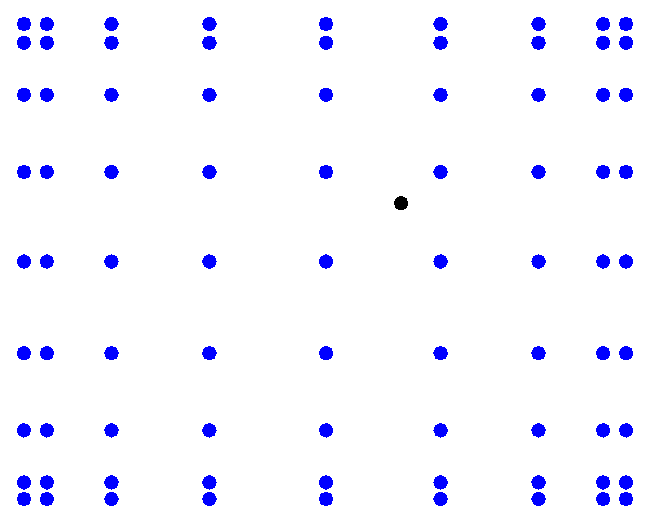
\includegraphics[scale = 0.5]{grid1.eps}
   \label{MERGEB}
 }\hfill
\subfloat[Chebyshev polynomials evaluated along the x-axis at the red points.]{
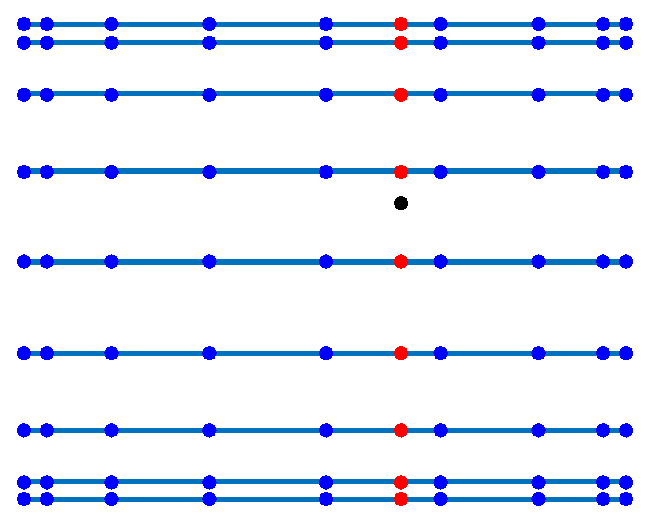
\includegraphics[scale = 0.5]{grid2.eps}
   \label{MERGEA}
 }
 
 \subfloat[Chebyshev polynomial evaluated along at the desired point.]{
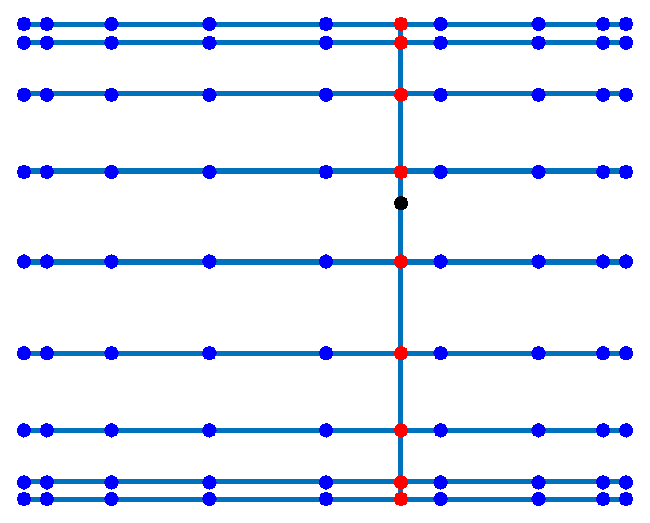
\includegraphics[scale = 0.5]{grid3.eps}
   \label{MERGEA}
 }
\caption{These pictures illustrate how we can computed multivariate Chebyshev interpolants using a one dimensional interpolation method.
}
\label{MULTI_INTERP}
\end{figure}

\section{Some Initial Results}
I have tested the our method on a  2D box with domain $[-1,1]x[-1,1]$. For the function
\begin{equation}
\arctan((x+y)/0.05),
\end{equation}
we have that our method takes 2.135446 seconds (with a splitting tolerance of 1e-14) while Chebfun2 takes 18 seconds.

For the function
\begin{equation}
\arctan(x/0.05)+\arctan(y/0.05),
\end{equation}
our method takes 1.4 seconds while Chebfun2 takes 0.1 seconds. Here is my initial though: Our method's complexity depends on how sharp the features of the function are while Chebfun2's complexity depends on the rank of the function.

\section{RASPEN Solver}
Here I lay out a plan for our to approach the Raspin Solver for a 1D BVP. Here, \bound{0}($\nu$),\bound{1}($\nu$) refer to the left and right interval points of interval($\nu$) as in our paper. The localsolve($\nu$,lbc,rbc) method solves the BVP locally on $\nu$ with the given boundary conditions; this is a method for leaves. The AlternatingSchwartz method would be called on non-leaves. This algorithm can be generalized to higher dimensions, but some care must be given to the boundaries. I will leave this for later.

\begin{algorithm}[!h]
\caption{v=AlternatingSchwartz($\nu$,lbc,rbc)}
\label{alg8}
\begin{algorithmic}
\IF{\child{0}($\nu$) is not a leaf}
\STATE $\hat{\text{rbc}}$ = evalf(\child{1}($\nu$),\bound{1}(\child{0}($\nu$)))
\STATE v0 = AlternatingSchwartz(\child{0}($\nu$),lbc,$\hat{\text{rbc}}$)
\ELSE
\STATE v0 = localsolve(\child{0}($\nu$),lbc,rbc)
\ENDIF

\IF{\child{1}($\nu$) is not a leaf}
\STATE $\hat{\text{lbc}}$ = evalf(\child{0}($\nu$),\bound{0}(\child{1}($\nu$)))
\STATE v1 = AlternatingSchwartz(\child{1}($\nu$),$\hat{\text{lbc}}$,rbc)
\ELSE
\STATE v1 = localsolve(\child{1}($\nu$),lbc,rbc)
\ENDIF
\STATE v = [v0;v1];
\end{algorithmic}
\end{algorithm}

For Algorithm~\ref{alg9}, the residuals of the BVP'S should be included in the nonlinear solve.

\begin{algorithm}[!h]
\caption{v=CourseSolve(T,$x_c$,$D_x$,$D_{xx}$,$u$)}
\label{alg9}
\begin{algorithmic}
\STATE sample(T,$u$)
\STATE [ubglob,udglobdx,uglobd2x] = evalf(T,points(T))
\STATE rglob = ODE(ubglob,udglobdx,uglobd2x)
\STATE $u_c$ = evalf(T,$x_c$)
\STATE $r_c$ = ODE($u_c$,$D_x u_c$, $D_{xx} u_c$)
\STATE sample(T,rglob)
\STATE g = rc - evalf(T,$x_c$)
\STATE v = fsolve(@(s) ODE($s$,$D_x s$,$D_{xx} s$)-g)
\end{algorithmic}
\end{algorithm}

We finally have the RASPEN iteration in \ref{alg10}.
\begin{algorithm}[!h]
\caption{F=Raspen($u$,T,$x_c$,$D_x$,$D_{xx}$,lbc,rbc)}
\label{alg10}
\begin{algorithmic}
\STATE $u_{\text{init}}=u$
\STATE v=CourseSolve(T,$x_c$,$D_x$,$D_{xx}$,$u$)
\STATE sample(T,v)
\STATE u = evalf(T,points(T))
\STATE Alt = AlternatingSchwartz(T,lbc,rbc)
\STATE sample(T,Alt)
\STATE F = evalf(T,points(T))
\end{algorithmic}
\end{algorithm}

\end{document}